
\section{Cel kompensacji}
\label{sec:cel_komp}

\subsection{Zastosowanie fal Lamba w nieniszczacych testach}

Fale prowadzone akustyczne i ultradźwiękowe, w tym między innymi fale Lamba, są wykorzystywane na wiele sposobów między innymi do nieniszczących testów oraz oceny jakości obiektów. Stosowane są między innymi do diagnostyki uszkodzeń aktywnych lub pasywnych w monitorowaniu kondycji strukturalnej (SHM - Structural Health Monitoring). W niektórych przypakach fale te są wykorzystywane do uzyskania lokalnych informacji o próbce, której to informacji nie można uzyskać konwencjonalnymi technikami ultradźwiękowymi. Przykładem takiego zastosowania może być inspekcja spoiwa klejowego \cite{kasia}. Jest to przykład aplikacji o krótkim zasięgu, ponieważ odległość propagacji fal kierowanych jest stosunkowo mała. Drugi obszar zastosowania kontroli fal prowadzonych jest przeznaczony do testowania dalekiego zasięgu. W tym przypadku odległość propagacji jest stosunkowo duża. Ich główną zaletą, sprawiającą, iż są one tak często wykorzystywane do diagnozy urządzeń jest to, że mogą być wzbudzane przez elementy uruchamiające znajdujące się na lub wewnątrz struktury w jednym punkcie konstrukcji i mogą się rozprzestrzeniać na duże odległości. Konwencjonalna kontrola ultradźwiękowa dużych struktur jest bardzo czasochłonna, ponieważ testom musi zostać poddany każdy punkt badanej struktury, która ma być monitorowana. Wykorzystanie fal Lamba jest więc potencjalnie bardzo atrakcyjnym rozwiązaniem tego problemu. Jeżeli przetwornik odbierający znajduje się w odległym punkcie struktury, odebrany sygnał zawiera informacje o całej przebytej ścieżce propagacji między przetwornikami nadawczym i odbiorczym. W związku z tym test monitoruje całą ściężkę, a nie pojedynczy punkt struktury. Pozwala to na znaczne zaoszczędzenie czasu badań. W przypadku prętów niejednokrotnie stosuje się techniki, w których nadajnik po wyemitowniu sygnału przełącza się w tryb odbiornika. Propagujący sygnał odbija się od końca pręta i wraca spowrotem, gdzie jest odbierany i może zostać poddany analizie. Takie podejście jest bardzo często stosowane, zwłaszcza w sytuacjach, w których dostęp do pręta możliwy jest tylko z jednej strony jak na przykład podczas badania kotw górniczych. Przykład ich położenia ilustruje rysunek \ref{fig:kotwy}
\begin{figure}[h]
\centering
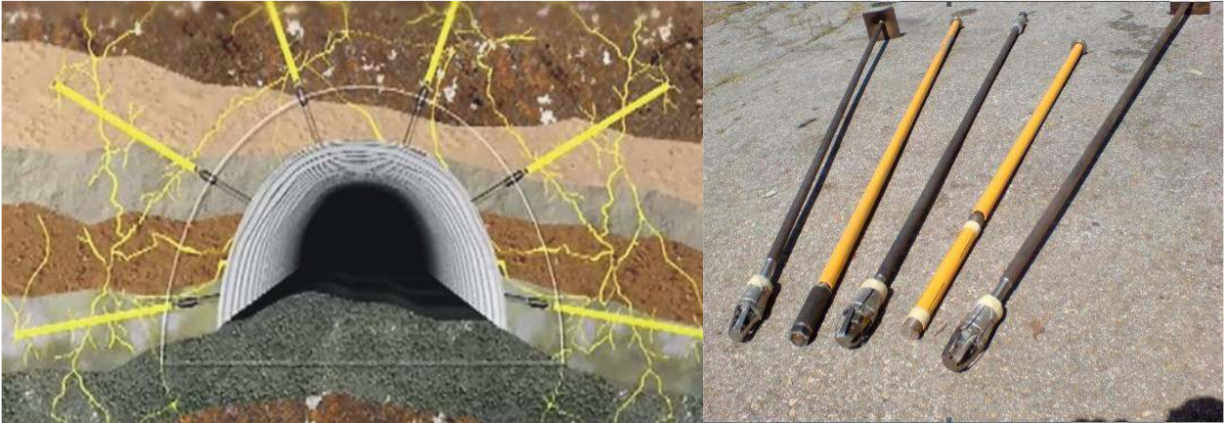
\includegraphics[width=14cm]{Zdjecia/4/kotwy}
\caption{Przykład zamontowania kotw górniczych, do których dostęp w przypadku testów jest tylko z jednej strony \cite{kotwy}}
\label{fig:kotwy}
\end{figure}

Nawet w najprostszych strukturach, takich jak swobodna płaska izotropowa płyta lub prosty stalowy pręt, może istnieć nieskończona liczba sterowanych trybów falowych. Co więcej, postaci te są generalnie dyspersyjne. Obydwa te fakty utrudniają praktyczne zastosowanie fal kierowanych. W praktyce testy kontroli dalekiego zasięgu są wykonywane w sposób zadowalający, gdy stosuje się tylko jedną lub czasami dwie postaci fal prowadzonych, a pozostałe są tłumione. Tradycyjnie osiąga się to za pomocą specjalnych przetworników. Dzięki starannej kontroli częstotliwości i liczby falowej wzbudzenia, możliwe jest generowanie wybranych postaci fali Lamba oraz tłumienie pozostałych. Kontrola zakresu częstotliwości może być osiągnięta przez użycie sygnału o pewnej szerokości pasma zamkniętego w oknie Hanninga lub Gaussa. Zakres liczby falowej może być ograniczony przez użycie starannie zaprojektowanych sond EMAT lub za pomocą piezoelektrycznego przetwornika. 

Powyższe metody mogą służyć do tłumienia sygnałów wywołanych przez niepożądane postaci fali, ale nie mogą zapobiec efektowi dyspersji, ponieważ zjawisko to występuje w falach kierowanych podczas ich propagacji w strukturze. Dyspersja sygnału powoduje, rozproszenie energii sygnału w czasie i przestrzeni w trakcie propagacji sygnału. W praktyce objawia się to wzrostem czasu trwania odbieranego sygnału w porównaniu do czasu trwania sygnału wejściowego. Rysunek \ref{fig:dyspersja} ilustruje przykład sygnału bez dyspersji oraz sygnału rozproszonego na skutek propagacji pewnej odległości. Łatwo zauważyć, że sygnał przed propagacją trwa zaledwie $0,0001 s$ natomiast po jego czas zwiększa się do około $0,0013s$ a zatem trwa ponad 10 razy dłużej.
\begin{figure}[h]
\centering
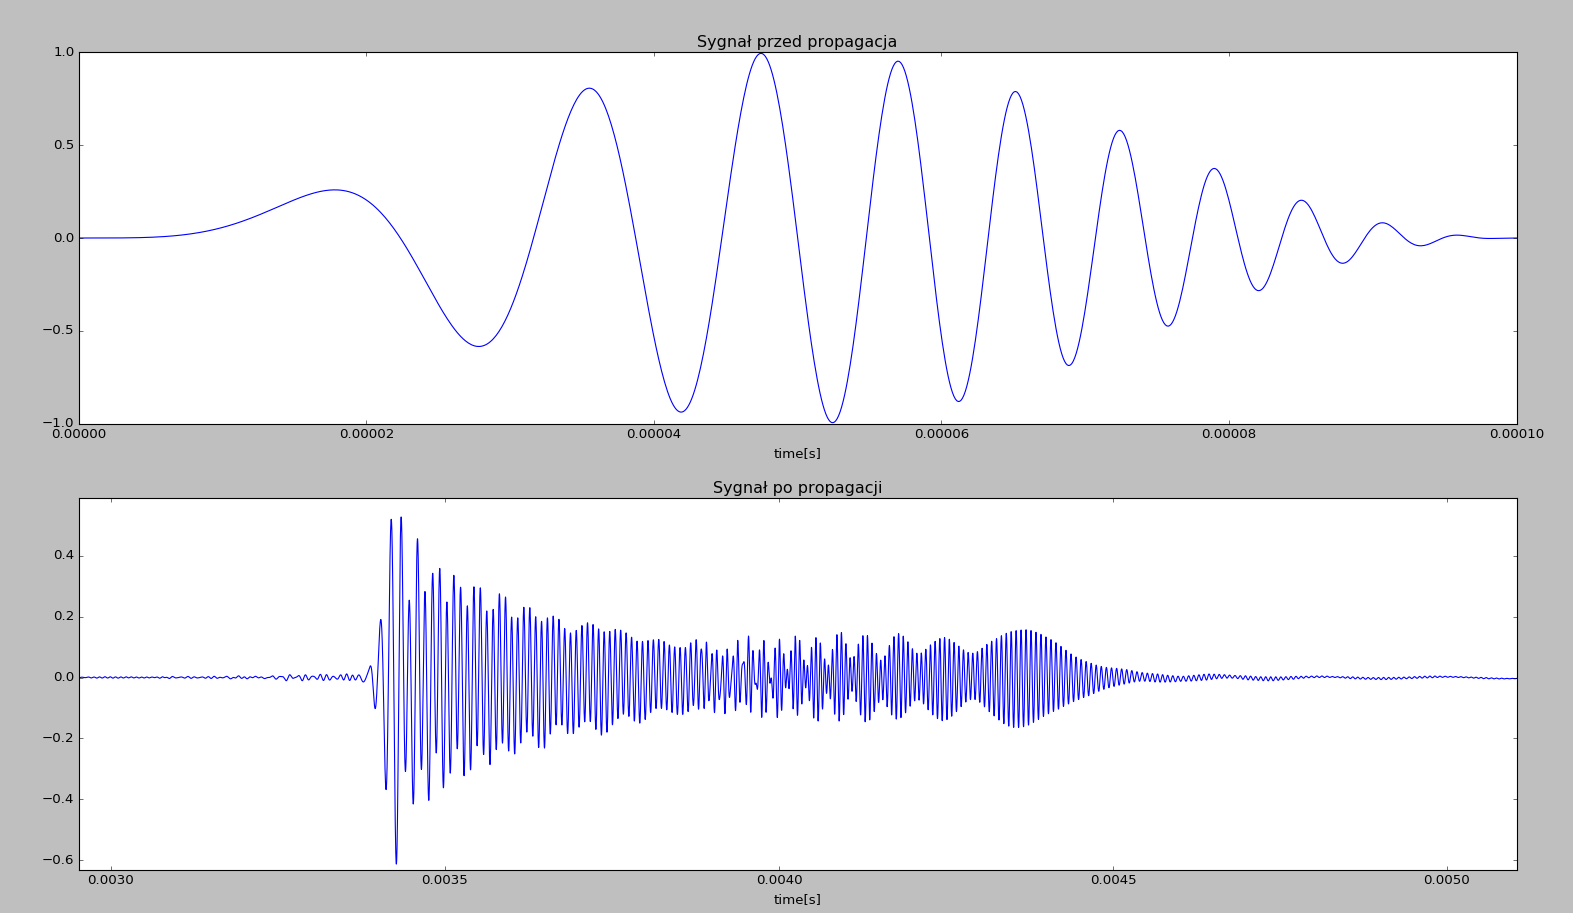
\includegraphics[width=14cm]{Zdjecia/4/dyspersja}
\caption{Przykład sygnału wejściowego, oraz sygnału rozproszonego}
\label{fig:dyspersja}
\end{figure}

 Zjawisko to pogarsza rozdzielczość i sprawia, że dane eksperymentalne są trudne do interpretacji z powodu nakładania się sygnałów. Używanie sygnałów wejściowych o określonej przepustowości może zmniejszyć problem dyspersji. Takie podejście koncentruje energię wejściową w ograniczonym zakresie częstotliwości, w którym jakiekolwiek zmiany prędkości pożądanego trybu fal kierowanych są małe. W praktyce oznacza to pracę w punktach na krzywych dyspersji dla konkretnego układu, w których prędkość grupowa jest stacjonarna lub prawie stacjonarna względem częstotliwości. Takie punkty zostały określone jako punkty "zerowej dyspersji" w \cite{kasia1}, jest to określenie, które może wprowadzać w błąd, ponieważ niemożliwe jest skoncentrowanie całej energii sygnału wejściowego o skończonej długości na jednej częstotliwości. Zostało udowodnione \cite{kasia2}, że istnieje optymalny sygnał wejściowy dla każdego punktu na krzywych dyspersji, który maksymalizuje rozdzielczość, jaką można uzyskać w tym punkcie. Jeśli jednak przyjmiemy, że przetwarzanie sygnału jest dozwolone przed wyświetlaniem informacji operatorowi, możliwe jest inne podejście do fal prowadzonych oraz ich roli w nieniszczących testach.

Należy również zaznaczyć, iż w praktyce rozproszone sygnały są zwykle uszkodzone z powodu szumów. Zachodzące na siebie i słabnące sygnały w porównaniu z szumem sprawiają, że dane z czujników są trudniejsze do interpretacji. W konsekwencji rodzielczość może ulec pogorszeniu. Dlatego zrodziła się ogromna potrzeba opracowania technik przetwarzania sygnałów w celu zwiększenia rozdzielczości czasowej i amplitudy SNR.

Z punktu widzenia systemów SHM, kompresja sygnału lub usuwanie dyspersji w dziedzinie czasu może być wygodnym i intuicyjnym sposobem na łatwiejszą interpretację sygnałów czujnika.

\subsection{Sygnał stosowany wy symulacji}
W ramach niniejszej pracy powstała aplikacja, pozwalająca użytkownikowi na podstawie podanych parametrów pręta wygenerować krzywe dyspersji opisujące dany obiekt. Aplikacja pozwala również na wygenerowanie sygnału testowego, symulację jego propagacji w zadanym pręcie, oraz kompensację otrzymanego sygnału wybranymi metodami. Sygnałem stosowanym do testów był sygnał chirp zmodyfikowany przypomocy okna Hanninga.
	Sygnał o nazwie chirp jest sygnałem sinusoidalnym, w którym faza jest funkcją czasu. \cite{kasia3}. Sygnał o nazwie linear chirp to sygnał, w którym częstotliwość zmienia się w sposób liniowo zależny od czasu. Sygnał taki jest opisany wzorem:
	\begin{equation}
	s(t) = \sin(\phi (t))
	\end{equation}
	
	Gdzie $\phi (t)$ to funkcja fazy. Chwilową częstotliwość takiego sygnału jest związana funkcją fazy następującą zależnością:
	\begin{equation}
	f(t) = \frac{1}{2\pi}\frac{d(\phi (t))}{dt} \label{eq:f(t)_z_phi}
	\end{equation}
	
	Aby zatem wygenerować sygnał linear chirp o rządanych parametrach należy przyjąć, iż funkcja częstotliwości przybiera postać:
	\begin{equation}
	f(t) = f_0+\frac{B}{T}t \label{eq:f(t)_liniowo}
	\end{equation}
	
	Gdzie:
	
	$f_0$ - częstotliwość początkowa
	
	$B$ - szerokość pasma częstotliwości
	
	$T$ - czas trwania sygnału
	
	Łącząc równania (\ref{eq:f(t)_z_phi}) oraz (\ref{eq:f(t)_liniowo}) można funkcję fazy zapisać jako:
	\begin{equation}
	\phi (t) = 2\pi f_0t+\frac{\pi Bt^2}{T} \label{eq:phi(t)}
	\end{equation}
	A zatem pełen wzór opisujący sygnał linear chirp można zapisać jako:
	\begin{equation}
	s(t) = \sin(2\pi f_0t+\frac{\pi Bt^2}{T})
	\end{equation}
	
	Przykład funkcji częstotliwości oraz uzyskanego w ten sposób sygnału przedstawia rysunek \ref{fig:linear_chirp}
\begin{figure}[h]
\centering
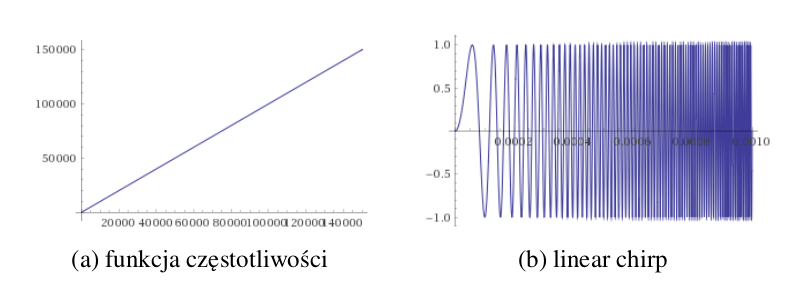
\includegraphics[width=14cm]{Zdjecia/4/linear_chirp}
\caption{Przykład sygnału linear chirp (b) oraz jego funkcji częstotliwości (a)}
\label{fig:linear_chirp}
\end{figure}

W prezentowanej pracy, sygnałem, który był poddawany symulacji był liniowy chirp dodatkowo pomnożony przez funkcję okna Hanninga daną wzorem:
\begin{equation}
w(n)=0,5(1-cos(\frac{2\pi n}{N-1})) \label{eq:okno_hanninga}
\end{equation}

Gdzie $N$ to całkowita liczba próbek. uzyskany w ten sposób sygnał został zaprezentowany na rysunku \ref{fig:test_chirp}
\begin{figure}[h]
\centering
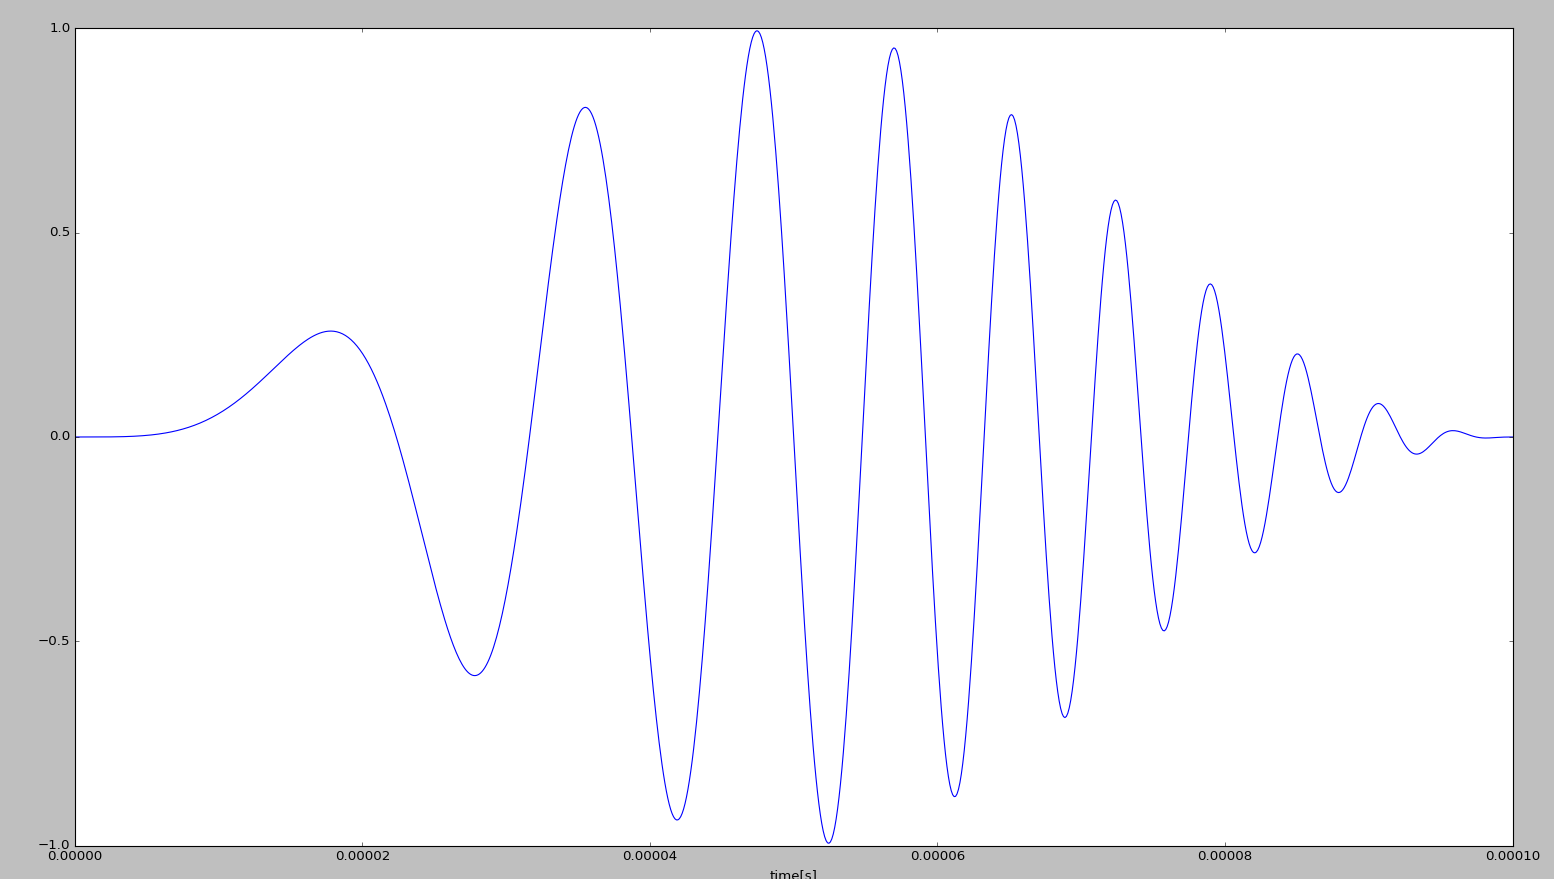
\includegraphics[width=14cm]{Zdjecia/4/test_chirp}
\caption{Linear chirp pomnożony przez funkcję okna Hanninga}
\label{fig:test_chirp}
\end{figure}

W aplikacji zaimplementowany został algorytm generujący opisany wyżej sygnał o następujących parametrach:

\begin{itemize}
\item czas trwania sygnału - 0.0001s
\item częstotliwość minimalna - 0Hz
\item częstotliwość maksymalna - 100kHz
\end{itemize}

Całość stworzona jest w oparciu o koncepcję otwartego kodu co daje użytkownikowi możliwość pisania własnych funkcji, generujących dowolne sygnały a następnie ich bezproblemową symulcję w stworzonej aplikacji.
